\chapter{Integration mit JavaScript}
\label{cha:JavaScript-Integration}

Im vorherigen Kapitel wurde gezeigt, wie das WebAssembly-Modul erzeugt wird. Grundsätzlich wäre dieses alleine lauffähig, funktioniert aber nicht, da Interaktion mit Ja\-va\-Script vorausgesetzt wird (zum Beispiel für Objektverwaltung, Konsolenausgaben und native Methoden), ist ein JavaScript-Gerüst rundherum notwendig, das alle Komponenten miteinander verbindet. Daher wird vom MiniJava-Compiler nicht nur ein einfache \lstinline{wasm}-Datei erzeugt, sondern ein Verzeichnis (im Quelltext \lstinline{Bundle} genannt, nachfolgend auch als \emph{Paket} bezeichnet) mit einigen JavaScript-Dateien und der \lstinline{wasm}-Datei.

\section{Aufbau des erzeugten Pakets}

Das Paket wird entsprechend der Struktur in Listing \ref{lst:bundle-structure} aufgebaut. Der Name des Wurzelverzeichnis ist beim Aufruf des MiniJava-Compilers frei wählbar, daher wurde er hier als Platzhalter mit \lstinline{<bundle-name>} gekennzeichnet. Alle mit einem \lstinline{(*)} gekennzeichnete Dateien sind von den zu kompilierenden Dateien abhängig und werden vom MiniJava-Compiler generiert. Alle anderen Dateien sind von den zu kompilierenden Dateien unabhängig und werden 1:1 in das Paket-Verzeichnis bei jedem Compileraufruf kopiert.

\lstinputlisting[label = {lst:bundle-structure}, caption = {Struktur des erzeugten Pakets}]{src/javaScriptIntegration/bundleStructure.txt}

\subsection{Kopierte Dateien}

Das Skript \emph{imports.js} ist für das Erstellen des Import-Objekts verantwortlich, das beim Instanzieren des WebAssembly-Moduls benötigt wird. Hier werden sowohl die Ja\-va\-Script-Im\-ple\-men\-tie\-rungen von sprachinternen Funktionalitäten als auch die Ja\-va\-Script-Pen\-dants nativer Methoden in ein Objekt zusammengefasst.

Das Skript \emph{internal.js} enthält die JavaScript-Implementierungen von sprachinternen Funktionalitäten für Felder und Zeichnketten-Konkatenationen.

Das Skript \emph{runtime.js} definiert in der JavaScript-Klasse \lstinline{Runtime} das Laufzeitsystem für das Zusammenspiel zwischen JavaScript und WebAssembly/MiniJava. In dieser Klasse befinden sich die Objektverwaltung und diverse Hilfsmethoden, um Daten zwischen JavaScript und WebAssembly/MiniJava auszutauschen und um von JavaScript ausgehend MiniJava-Methoden aufrufen zu können.

\subsection{Generierte Dateien}

Alle JavaScript-Pendants für native Methoden werden in das Verzeichnis \emph{native} kopiert. Um dabei potenzielle Dateinamenkollisionen zu umgehen, werden alle Dateien ab 0 beginnend nummeriert.

Der generierte Bytecode wird in der Datei \emph{module.wasm} abgelegt. Als Zwischenprodukt entsteht beim Kompilieren die Datei \emph{module.wat}, die lediglich die textuelle Repräsentation des WebAssembly-Moduls darstellt\footnote{Der Grund dafür ist, dass das Erstellen der textuellen Repräsentation wesentlich einfacher ist. Außerdem können beim Entwickeln des Compilers potenzielle Fehler leichter in einer Textdatei als in einer binären Datei gefunden werden.}. Aus dieser Datei entsteht mit dem Werkzeug \lstinline{wat2wasm} \cite{WABT} dann die binäre Form des Moduls. Die textuelle Repräsentation wird zur Laufzeit grundsätzlich nicht benötigt.

Alle im MiniJava-Quelltext vorhandenen Zeichenketten-Literale werden in der Datei \emph{module.js} registriert. Außerdem werden zur Compile-Zeit sämtliche Konstrukturen, \emph{Getter} und \emph{Setter} für MiniJava-Klassen generiert und in dieser Datei gespeichert. Weiters referenziert diese Datei alle JavaScript-Dateien im Verzeichnis \emph{native}.

\subsection{Zusammenhang zwischen den Dateien}

Je nachdem, auf welcher Plattform das Paket ausgeführt wird, muss das WebAssembly-Modul unterschiedlich geladen werden: Bei Node.js kann das Modul direkt aus dem Dateisystem gelesen werden, im Browser muss es von einem Web-Server heruntergeladen werden. Um für die verschiedenen Einsatzgebiete Flexibilität zu ermöglichen, wird das WebAssembly-Modul nicht direkt von den anderen JavaScript-Dateien referenziert. In Abbildung \ref{fig:bundleStructure} wird der Zusammenhang zwischen den JavaScript-Dateien visualisiert.

\begin{figure}[]
    \centering
    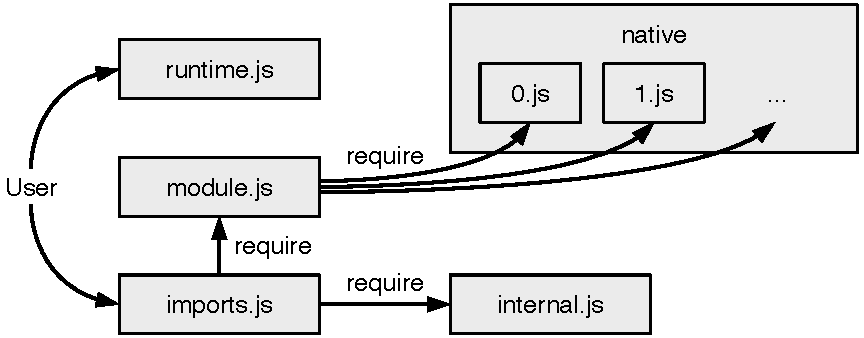
\includegraphics[width=0.8\textwidth]{javaScriptIntegration/bundle}
    \caption{Zusammenhang der JavaScript-Dateien in einem Paket}
    \label{fig:bundleStructure}
\end{figure}

Auf die praktische Verwendung des gesamten Pakets wird in diesem Kapitel nicht eingangen. Im Abschnitt \ref{sec:NodeJSExample} wird anhand eines Beispiels gezeigt, wie sich das Paket in eine Node.js-Konsolenanwendung integrieren lässt.

\section{JavaScript-Codegenerierung}
\label{sec:JavaScript-Codegenerierung}

Wie im vorherigen Abschnitt beschrieben, wird beim Kompilieren Ja\-va\-Script-Quell\-text in der Datei \emph{module.js} generiert.

Beim Erzeugen des Bytecodes wurden bereits für die Zeichenketten-Literale Referenzen (ab 1 beginnend) festgelegt. Daher müssen später zur Laufzeit die Zeichenketten-Literale in der Reihenfolge der zuvor zugewiesenen Referenzen (siehe Abschnitt \ref{subsec:Zeichenketten-Literale}) registriert werden. Dies muss erfolgen, bevor das WebAssembly-Modul gestartet wird, da zu diesem Zeitpunkt noch keine Objekte erstellt wurden. So wird garantiert, dass sich die Referenzen nicht verschieben.

Außerdem muss für jede Klasse ein Konstruktur generiert werden. Dieser hat die Aufgabe, ein JavaScript-Objekt zu erzeugen, in dem alle Datenkomponenten mit einem (je nach Datentyp) sinnvollen Platzhalterwert initialisiert werden. Außerdem wird der entsprechende MiniJava-Datentyp mit dem Objekt verknüpft. Die Konstrukturen liefern als Rückgabewert eine Referenz des erzeugten Objekts.

Datenkomponenten von MiniJava-Klassen werden direkt auf Datenkomponenten von Java\-Script-Objekten abgebildet. Da WebAssembly nicht direkt auf JavaScript-Objekte zugreifen kann, müssen für diese \emph{Getter} und \emph{Setter} erzeugt werden, die diese Aufgabe übernehmen. Die \emph{Getter} bekommen als Parameter nur die Referenz des Objekts und müssen den Wert der Datenkomponente (oder eine Referenz darauf wenn die Datenkomponente ein Objekt referenziert) zurückgeben. Ähnlich funktionieren die \emph{Setter}: Diese bekommen zwei Parameter, die Referenz des Objekts und den Wert des neuen Werts für die Datenkomponente (oder eine Referenz, wenn es sich um Objekte handelt). \emph{Setter} haben keinen Rückgabewert.

\pagebreak
Die Codegenerierung wird anhand eines überschaubaren Beispiel nun detailliert gezeigt. Nachfolgend ist der MiniJava-Quelltext für dieses Beispiel dargestellt:

\lstinputlisting{src/javaScriptIntegration/Example.minijava}

Aus diesem Quelltext wurde vom Compiler die Datei \emph{module.js} generiert:

\lstinputlisting{src/javaScriptIntegration/module.js}

Nachfolgend einige Details zur generierten Datei:

\begin{itemize}
    \item In den Zeilen 2 und 3 werden die Zeichenketten-Literale registriert. 
    \item In den Zeilen 7 bis 9 befindet sich der Konstruktor der Klasse \lstinline{MyClass}, der die Datenkomponenten mit \lstinline{0} und \lstinline{null} initialisiert.
    \item In den Zeilen 3 bis 15 werden \emph{Getter} und \emph{Setter} für die \lstinline{int}-Datenkomponente definiert. Da es sich um einen elementaren Datentyp handelt, kann der Wert direkt aus dem übergebenen Parameter gelesen werden (\emph{Setter}) bzw. als Rückgabewert geliefert werden (\emph{Getter}).
    \item In den Zeilen 16 bis 21 werden \emph{Getter} und \emph{Setter} für die \lstinline{String}-Datenkomponente definiert. Hier muss der Parameter beim \emph{Setter} zunächst derefenziert werden bzw. muss beim \emph{Getter} zunächst eine Referenz auf das Objekt erzeugt werden.
\end{itemize}

\section{Objektverwaltung für MiniJava in JavaScript}

Sämtliche Objekte, auf die von MiniJava zugegriffen wird, werden in JavaScript als echte JavaScript-Objekte verwaltet. Diese Objekte werden in MiniJava über eine Referenz angesprochen. Im Wesentlichen entspricht diese Referenz einer fortlaufenden Nummer, die bei 1 beginnt, da 0 \lstinline{null} entspricht.

Es muss möglich sein, eindeutig von einem Objekt auf die Referenz und umgekehrt schließen zu können. Für beide Richtungen wird diese Abbildung jeweils mit einer Java\-Script-\lstinline{Map} realisiert.

Diese \lstinline{Maps} werden in der JavaScript-Klasse \lstinline{Runtime} verwaltet. Im Konstruktor werden diese sinnvoll initialisiert, beispielsweise wird die Referenz 0 auf \lstinline{null} und umgekehrt abgebildet:

\lstinputlisting{src/javaScriptIntegration/runtimeConstructor.js}

Weiters werden drei Methoden zur Verfügung gestellt, zwei für das Erstellen einer Referenz auf ein JavaScript-Objekt und eine für das Dereferenzieren einer Referenz:
\begin{enumerate}
    \item Die Methode \lstinline{wasmRef} liefert die Referenz auf das Objekt, falls bereits eine Referenz erstellt wurde oder erstellt eine neue, falls das Objekt noch keine Referenz besitzt.
    \item Die Methode \lstinline{wasmRefType} liefert ebenfalls die Referenz auf das Objekt. Sie sollte genau dann verwendet werden, wenn das erste Mal eine Referenz für ein Ja\-va\-Script-Ob\-jekt angefordert wird, da hier der MiniJava-Datentyp des Objekts registriert wird. Dieser Typ wird später für Methodenaufrufe benötigt.
    \item Die Methode \lstinline{wasmDeref} liefert \lstinline{wasmDeref} das Objekt bzw. \lstinline{null} hinter der Referenz.
\end{enumerate}

Nachfolgend wird der Quelltext für diese drei Methoden dargestellt:

\lstinputlisting{src/javaScriptIntegration/runtimeRefs.js}

\section{Hilfsmethoden}

Die Klasse \lstinline{Runtime} bietet noch einige nützliche Hilfsmethoden an, die das Zusammenspiel zwischen JavaScript und WebAssembly/MiniJava erleichtern sollen:

\lstinputlisting{src/javaScriptIntegration/runtimeHelpers.js}

Mit \lstinline{wasmBoolean} kann ein Wert des MiniJava-Datentyps \lstinline{boolean} (entspricht einer Ganzahl in WebAssembly) in Wert des JavaScript-Datentyps \lstinline{boolean} konvertiert werden. In die andere Richtung ist keine explizite Konvertierung erforderlich.

Mit \lstinline{charToWasm} und \lstinline{wasmToChar} kann zwischen einem Wert des MiniJava-Datentyps \lstinline{char} (entspricht ebenfalls einer Ganzzahl in WebAssembly) und einem Wert des Ja\-va\-Script-Da\-ten\-typs \lstinline{string} mit genau einem Zeichen konvertiert werden.
Es muss der JavaScript-Datentyp \lstinline{string} verwendet werden, da JavaScript keinen eigenen Datentyp für einzelne Zeichen besitzt.

\section{Sprachinterne Funktionalitäten}
\label{sec:Sprachinterne-Funktionalitäten}

MiniJava bietet einige Sprachfunktionalitäten an, die nicht zur Gänze in WebAssembly abgebildet werden können, da sie mit JavaScript-Objekten interagieren. Dazu zählen alle Funktionalitäten rund um Felder wie das Erstellen eines Felds, das Abfragen der Länge des Felds und das Zugreifen über einen Index. Außerdem bietet MiniJava das Konkatenieren von Zeichenketten an.

\subsection{Feld-Funktionen}
\label{subsec:Feld-Funktionen}

Die Implementierung der Feld-Funktionen sind vom konkreten Element-Datentyp des Felds abhängig. Allgemein lassen sich daher vier Fälle unterscheiden:

\begin{enumerate}
    \item Werte numerische Datentypen wie \lstinline{int} und \lstinline{float} werden auf denselben Ja\-va\-Script-Da\-ten\-typ abgebildet, da JavaScript nur den Datentyp \lstinline{number} für numerische Werte zur Verfügung stellt.
    \item Werte des \lstinline{boolean}-Datentyps müssen zwischen JavaScripts \lstinline{true} und \lstinline{false} auf 1 und 0 und umgekehrt abgebildet werden, da WebAssembly keinen eigenen Datentyp für Wahrheitswerte besitzt
    \item Werte des \lstinline{char}-Datentyps müssen zwischen einer Ganzzahl und einem Zeichenkette mit einem Zeichen abgebildet werden.
    \item Objekte  müssen auf Referenzen und umgekehrt abgebildet werden. 
\end{enumerate}

Sämtliche Funktionen für Felder wurden für diese vier Fälle einzeln implementiert und funktionieren ähnlich. Im WebAssembly-Modul werden die Funktionen über einen Funktionsnamen importiert, der folgendem Schema entspricht: \\
\lstinline{<function>_array_<type>}

Am interessantesten sind die Funktionen für Felder von Objekten, daher werden diese nun im Detail betrachtet.

Beim Erstellen eines Felds wird ein JavaScript-Feld in der angeforderten Größe erstellt und mit Standardwerten (hier \lstinline{null}) vorbefüllt:
\lstinputlisting{src/javaScriptIntegration/arrayNew.js}

Das Abrufen eines Objekts über den Index funktioniert so, dass zunächst das Array selbst derefenziert werden muss. Anschließend wird für das über den Index erhaltene Objekt mit \lstinline{runtime.wasmRef} eine Referenz erstellt:
\lstinputlisting{src/javaScriptIntegration/arrayGet.js}

Analog dazu funktioniert das Setzen eines Objekts mit einem Index:
\lstinputlisting{src/javaScriptIntegration/arraySet.js}

Die Funktion für das Abfragen der Länge des Felds ist typunabhängig, daher gibt es dafür nur eine Implementierung:

\lstinputlisting{src/javaScriptIntegration/arrayLength.js}

\subsection{Zeichenketten-Konkatenation}
\label{subsec:JavaScript-Zeichenketten-Konkatenation}

Alle Verwendungen des MiniJava-Konkatenationsoperators \lstinline{+} werden auf JavaScript-Funktionen abgebildet. Dabei muss zumindest auf einer Seite des Operators ein Mi\-ni\-Ja\-va-\lstinline{String} stehen. Abhängig vom Datentyp auf der anderen Seite des Operators gibt es (ähnlich wie bei den Feldern) eine eigene Implementierung. Im WebAssembly-Modul werden die Funktionen über einen Funktionsnamen importiert, der folgendem Schema entspricht: \\
\lstinline{+_<left-type>_<right-type>}

Die erste Variante ist das Konkatenieren von zwei Zeichenketten. Hier werden zunächst die Referenzen der beiden Zeichenketten dereferenziert. Anschließend wird eine Referenz auf die zusammengesetzte Zeichenkette erstellt:
\lstinputlisting{src/javaScriptIntegration/stringString.js}

Die zweite Variante ist Konkatenieren von einer Zeichenkette mit dem Wert eines anderen Datentyps \emph{T}. Der Datentyp \emph{T} kann entweder auf der rechten oder linken Seite des Operators stehen, das ergibt zwei Möglichkeiten pro Datentyp. Ähnlich wie bei den Feldern gibt es dieselben vier Fälle für den Datentyp \emph{T}. Jede Kombination wird in einer eigenen Funktion implementiert, insgesamt ergibt das somit acht Funktionen. Der Wert des Datentyp \emph{T} wird dabei automatisch in eine Zeichenkette umgewandelt.

Da das Konkatenieren für die einzelnen Datentypen ähnlich funktioniert, werden stellvertretend nun beispielhaft die zwei Funktionen gezeigt, um einen Zeichenkette mit einem numerischen Wert zu verketten:
\lstinputlisting{src/javaScriptIntegration/stringNumeric.js}

\section{Methodenaufrufe von JavaScript nach MiniJava}

Alle MiniJava-Methoden, die mit dem Schlüsselwort \lstinline{public} gekennzeichnet wurden, werden als Funktion im WebAssembly-Modul exportiert, siehe Abschnitt \ref{sec:Exportieren-von-Methoden}.

In der JavaScript-Klasse \lstinline{Runtime} wird die Funktion \lstinline{findMethod} zur Verfügung gestellt, die aus dem Klassennamen, dem Methodennamen und der Liste der Eingabeparametertypen den exportierten WebAssembly-Funktionsnamen ableitet. Anschließend wird die Funktion aus der \lstinline{exports}-Datenstruktur der WebAssembly-Modulinstanz abgerufen.

\pagebreak
\lstinputlisting{src/javaScriptIntegration/runtimeFindMethod.js}

Auf dieser Funktion aufbauend können nun Aufrufe auf Klassenmethoden und Objektmethoden realisiert werden.

\subsection{Aufruf von Klassenmethoden}

Bei Aufrufen von Klassenmethoden kann \lstinline{findMethod} direkt verwendet werden. Um die Schnittstelle der \lstinline{Runtime}-Klasse zu vereinheintlichen, wird der Aufruf von \lstinline{findMethod} in der Methode \lstinline{staticMethod} gekapselt, dies spiegelt die Kennzeichnung im MiniJava-Quelltext durch das Schlüsselwort \lstinline{static}.

\lstinputlisting{src/javaScriptIntegration/runtimeStaticMethod.js}

Nun kann eine Klassenmethode aufgerufen werden. So wird beispielsweise die Mini\-Java-Methode \lstinline{public static int add(int a, int b)} der MiniJava-Klasse \lstinline{Utils} in Java\-Script mit den Parametern \lstinline{a = 3} und \lstinline{b = 4} aufgerufen:

\lstinputlisting{src/javaScriptIntegration/staticCall.js}

\subsection{Aufruf von Objektmethoden}

Objektmethoden können nicht wie Klassenmethoden aufgerufen werden, da zunächst der Typ des Objekts, für welches die Methode aufgerufen wird, bestimmt werden muss. Damit dies möglich ist, muss das Empfängerobjekt bereits mit \lstinline{runtime.wasmRefType} registriert sein. Anschließend kann mit \lstinline{findMethod} die Methode gesucht werden. Da Objektmethoden per Konvention als ersten Parameter eine Referenz auf das Empfängerobjekt erwarten (\lstinline{this}-Parameter, siehe Abschnitt \ref{subsec:this-Parameter}), muss die Referenz als erster Parameter beim Aufruf eingefügt werden:

\lstinputlisting{src/javaScriptIntegration/runtimeInstanceMethod.js}

Da die Anzahl der Parameter von der tatsächlichen Methode abhängig ist, werden in Zeile 4 beim Lambda-Ausdruck in der Parameterliste \emph{Rest-Parameter} (\lstinline{...args}) \cite{MDNJavaScript} verwendet, die alle übergebenen Parameter in der Liste \lstinline{args} speichern. Beim Aufruf der WebAssembly-Funktion muss diese Parameterliste wieder ausgepackt werden, ansonsten würde man die Parameterliste als ein Listenobjekt übergeben. Dafür wird die \emph{Spread-Syntax} (\lstinline{...args}) verwendet. Die beiden Konstrukte sind syntaktisch ident, erfüllen aber die jeweils gegensätzliche Funktion.

Nun kann ein Aufruf einer Objektmethode durchgeführt werden. So wird beispielsweise die MiniJava-Methode \lstinline{public void increment(int a)} eines Objekts \lstinline{obj} in JavaScript mit dem Parameter \lstinline{a = 3} aufgerufen:

\lstinputlisting{src/javaScriptIntegration/instanceCall.js}

\section{Standardbibliothek}
\label{sec:Standardbibliothek}

Moderne Programmiersprache benötigt eine Standardbibliothek. Diese sollte einerseits Basisfunktionalitäten zur Verfügung stellen, um sinnvoll mit der Laufzeitumgebung interagieren zu können. Andererseits können hier oft verwendete Basisfunktionalitäten zur Verfügung gestellt werden, die in nahezu jeder Anwendung benötigt werden.

Um einen Eindruck zu vermitteln, wie man für MiniJava die Grundsteine für eine Standardbibliothek legen könnte, wurden einige solche Basisfunktionalitäten implementiert. In diesem Abschnitt werden einige Ausschnitte daraus präsentiert.

Bei Interaktionen mit der Laufzeitumgebung sind native Methoden mit JavaScript-Pendants unumgänglich. Somit vermittelt dieser Abschnitt ebenfalls einen Einblick dafür, wie native Methoden aufgebaut werden können.

\subsection{Konsolenausgabe}
Die einfachste Form einer Benutzeroberfläche ist die Konsole. Daher ist die Konsole die absolute Grundvoraussetzung, um die Ergebnisse eigener Programme sehen zu können.

Sämtliche Funktionalitäten für die Konsolenausgabe wurden in der MiniJava-Klasse \lstinline{Console} gekapselt, die eine Reihe an Klassenmethoden zur Verfügung stellt. Hier werden nur zwei davon gezeigt, in der vollständigen Implementierung sind noch weitere mehr vorhanden, wie zum Beispiel zur Ausgabe von Feldern. In MiniJava werden die Methoden für die Konsolenausgabe folgendermaßen definiert:
\lstinputlisting{src/javaScriptIntegration/Console.minijava}

In JavaScript werden die Aufrufe an \lstinline{console.log} delegiert:
\lstinputlisting{src/javaScriptIntegration/Console.js}

\subsection{Methoden für den Datentyp \lstinline{String}}

Zeichenketten sind ein notwendiger Basisdatentyp in jeder Programmiersprache. Zu den Basisfunktionalitäten für Zeichenketten zählen das Bestimmen der Länge, das Abfragen eines Zeichens an einer Stelle und der Vergleich, ob zwei Zeichenketten gleich sind.

Diese drei Funktionalitäten werden als Objektmethoden in der MiniJava-Klasse \lstinline{String} definiert:
\lstinputlisting{src/javaScriptIntegration/String.minijava}

In JavaScript werden diese Methoden mit Hilfe von bereits bestehenden Funktionalität implementiert:
\lstinputlisting{src/javaScriptIntegration/String.js}

\subsection{Konvertieren zwischen Ganzzahlen und Zeichenketten}

Oft werden zum Beispiel in der Konsole oder in einer grafischen Benutzeroberfläche Zahlen eingegeben. Diese stehen dann in Form von Zeichenketten zur Verfügung. Um mit den Werten sinnvoll arbeiten zu können, müssen die Zeichenketten in Zahlen konvertiert werden. Umgekehrt müssen Zahlen zum Beispiel für Ausgaben wiederum in Zeichenketten konvertiert werden.

Dafür wurden (angelehnt an die Java-Standardbibliothek) zwei Klassenmethoden in der MiniJava-Klasse \lstinline{Integer} definiert:
\lstinputlisting{src/javaScriptIntegration/Integer.minijava}

\pagebreak
Da JavaScript auch dafür bereits Funktionalitäten zur Verfügung stellt, wird das Konvertieren an JavaScript delegiert:
\lstinputlisting{src/javaScriptIntegration/Integer.js}

\vspace{4em}
In diesem Kapitel wurde beschrieben, wie ein Paket aufgebaut ist und welche Rolle die einzelnen JavaScript-Dateien darin spielen. Weiters wurde auf das in JavaScript implementierte Laufzeitsystem eingegangen, dabei wurde der Fokus auf Objekt-Verwaltung, Felder und Zeichenketten gelegt. Zum Schluss wurde gezeigt, wie JavaScript mit MiniJava-Methoden interagieren kann.

Somit sind nun alle Grundlagen des Compilers abgeschlossen. Im nächsten Kapitel wird auf das Testen des Compilers eingegangen. Außerdem wird das Integrieren in Gradle gemeinsam mit dem Einsatz des Compilers in einer Konsolenanwendung gezeigt.
